\begin{frame}[plain,c]
\begin{center}
	\huge Important remark
\end{center}
\end{frame}

\begin{frame}
	\pause[1]
	\begin{theorem}
		If a $(v,k,\lambda)-BIBD$ exist, then $\lambda(v-1) \equiv 0 (mod(k-1))$ and $\lambda v(v-1) \equiv (mod k(k-1))$.
	\end{theorem}
	
	\pause[2]
	Only \textbf{necessary}.
	
	\pause[1]
	\begin{theorem}
		A STS of \textit{order} $v$ \textbf{exists} if and only if $v\equiv 1,3\ mod(6)$  
	\end{theorem}
	
	\pause[2]
	\textbf{Necessary} and \textbf{sufficient}.
\end{frame}
\begin{frame}
\frametitle{STS on OEIS}
\begin{figure}
	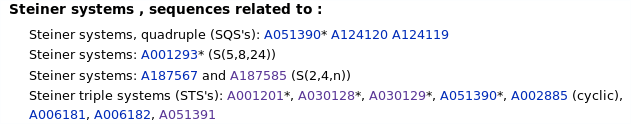
\includegraphics[width=1\textwidth]{oeis_on_sts}
\end{figure}
\end{frame}

\begin{frame}
\frametitle{Isomorphisms between two \textit{design}}
\begin{block}{Isomorphism}
Two designs $(X,\mathrm{A})$ and $(Y,\mathrm{B})$ where $|X|=|Y|$ are \textit{isomorphic} if there \textit{exists} a bijection $\alpha : X \rightarrow Y$ such that:
\begin{center}
	\begin{math}
	\{ \alpha(x) : x \in A \} = \mathrm{B}
	\end{math}%In other words, if we rename every point x ∈ X by α(x), then the collection of blocks
	% is transformed into B. The bijection α is called an isomorphism.

\end{center}	
Then $\alpha$ is called isomorphism.
\end{block}
\begin{figure}
	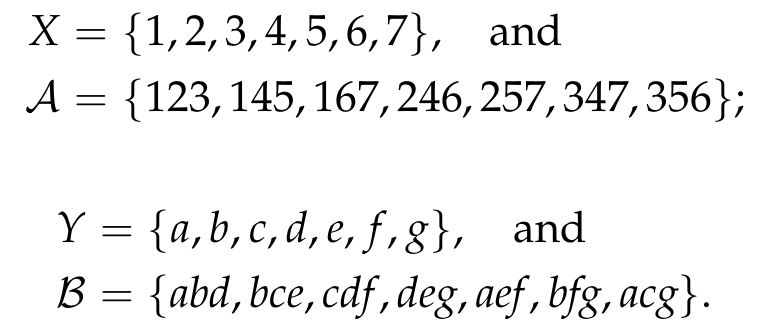
\includegraphics[width=0.65\textwidth]{isomorphism}
\end{figure}
\end{frame}

%due sts non-isomorfi quindi sono sts che hanno lo stesso ordine ma che una funzione biunivoca non riesce a mappare, effettivamente sono diversi quindi.
\begin{frame}
	\frametitle{Beyond Existence or non-existence}
	
\begin{columns}
\column[]{0.5\textwidth}
\begin{table}[]
\begin{tabular}{cccll}
\cline{1-2}
\multicolumn{1}{|c|}{} & \multicolumn{1}{c|}{$t_1$}  &  &  \\ \cline{1-2}
\multicolumn{1}{|c|}{1} & \multicolumn{1}{c|}{1}  &  &  \\ \cline{1-2}
\multicolumn{1}{|c|}{2} & \multicolumn{1}{c|}{1}  &  &  \\ \cline{1-2}
\multicolumn{1}{|c|}{3} & \multicolumn{1}{c|}{1}   &  \\ \cline{1-2}
\multicolumn{1}{l}{}    & \multicolumn{1}{l}{}      &  & 
\end{tabular}
\caption{Incidence matrix of STS(3)}
\end{table}	
\column[]{0.5\textwidth}
\begin{block}{Incidence matrix}
Fixed a design $(S,T) \equiv (\{s_1, ..., s_{|S|} \},\{t_1, ..., t_{|T|} \})$ let all elements $m_{i,j}$ of \textit{incidence matrix} of a design $(S,T)$ be:

\begin{math}
m_{i,j} = 
\begin{cases*}
1 & if $s_i \in t_j$\\
0 & if $s_i \not \in t_j$
\end{cases*}
\end{math}

\end{block}
\end{columns}


\end{frame}

\begin{frame}
\frametitle{2-isomorphic sts(7)}
$v=7$,\quad $k=\binom{7}{2}/3$

\begin{columns}
	\column[]{0.5\textwidth}
	\begin{table}
		\begin{tabular}{|l|l|l|l|c|c|c|}
			\hline
			1 & 2 & ~ & 4 & ~ & ~ & ~ \\ \hline
			~ & 2 & 3 & ~ & 5 & ~ & ~ \\ \hline
			~ & ~ & 3 & 4 & ~ & 6 & ~ \\ \hline
			~ & ~ & ~ & 4 & 5 & ~ & 7 \\ \hline
			1 & ~ & ~ & ~ & 5 & 6 & ~ \\ \hline
			~ & 2 & ~ & ~ & ~ & 6 & 7 \\ \hline
			1 & ~ & 3 & ~ & ~ & ~ & 7 \\ \hline
		\end{tabular}
	\end{table}

	\column[]{0.5\textwidth}
	\begin{table}[]
		\begin{tabular}{|c|c|c|c|c|c|c|}
			\hline
			&   &   &   & 5 & 6 & 7 \\ \hline
			&   & 3 & 4 &   &   & 7 \\ \hline
			1 & 2 &   &   &   &   & 7 \\ \hline
			& 2 &   & 4 &   & 6 &   \\ \hline
			1 &   & 3 &   &   & 6 &   \\ \hline
			& 2 & 3 &   & 5 &   &   \\ \hline
			1 &   &   & 4 & 5 &   &   \\ \hline
		\end{tabular}
	\end{table}
\end{columns}
\end{frame}


\begin{frame}
\setbeamercolor{block title}{bg=red!30,fg=black}
\pause[1]
\begin{block}{}
The enumeration of non-isomorphic STS is complex and a open field.
\end{block}

%faccio un esempio -> quanti sono ? -> primo non-isomoprhic -> stima di Wilson 1974 -> stima di Stinson 1985

\setbeamercolor{block title}{bg=blue!30,fg=black}
\pause[2]
\begin{block}{(A030129) Number of nonisomorphic Steiner triple systems (STS's) $S(2,3,n)$ on $n$ points}
	$<1, 0, 1, 0, 0, 0, 1, 0, 1, 0, 0, 0, 2, 0, 80, 0, 0, 0, 11084874829>$%fino a 19 e il primo che ne ha 2 è 9
\end{block}
\begin{block}{(A051390)Number of nonisomorphic Steiner quadruple systems (SQS's) of order $n$ }
	$<1, 1, 0, 1, 0, 0, 0, 1, 0, 1, 0, 0, 0, 4, 0, 1054163>$%16
\end{block}
\end{frame}

\begin{frame}
\frametitle{[1974 Wilson]Upper bound to non-isomorphic STS(v)}
A algebric result:
\begin{center}
	\begin{math}
		F(v) \le ((1 + o (1)\frac{v}{e^2})^{\frac{n^2}{6}}
	\end{math}
\end{center}
\end{frame}


\begin{frame}
\frametitle{[1985 Stinson]Estimation of STS(19)}
Was discovered 284457 non-isomorphic through different methods.
They had discovered $N(19) \ge 2395687$  through a \textit{non-deterministic hill-climbing algorithm}. Then for every STS(19) calculate 2 \textit{invariants} (non-isomorphic give the property of different invariant.) First they conclude $N=3.54 \times 10^8$, but the random seed was from a population of $10^9$($11084874829$) and some 2 isomorphic STS may have the same invariants.\\

They made another estimation by knowing the \textit{right number} of $sub-STS(9)$ the $N(19)$ by looking the ratio of of $sub-STS(9)$ fount divided by the right times the number of nonisomorphic sts. So... they \textcolor{red}{miss by an order of magnitude} but really close!.
\end{frame}